\section{L'utilisation de la cryptographie dans la vie quotidienne}
Au travers de ce chapitre, nous allons voir quelques utilisations
quotidiennes de la cryptographie.
 
\subsection{Login système}
Commençons par le commencement : lorsqu'on allume un ordinateur,
et qu'on s'identifie (on se \emph{log}), il faut, dans la plupart 
des cas, entrer un mot de passe (bien que cette fonctionnalité
ne soit est plus activée par défaut sur les systèmes d'exploitation
Windows, elle reste fortement conseillée).
\\
 
Sous les systèmes bade type UNIX, le programme qui se charge de
l'identification est \texttt{login} (lancé directement après
\texttt{init} et \texttt{getty}). À la base, les mots de passe
étaient stockés en clair dans le fichier \texttt{/etc/passwd},
mais se trouvent désormais chiffrés dans un autre
fichier (\texttt{/etc/shadow} sous Linux,
\texttt{/etc/master.passwd} sous FreeBSD, …), 
lisible uniquement par le «~super utilisateur~»
(l'utilisateur \texttt{root}).
Les algorithmes de chiffrements
utilisés sont des algorithmes dérivés de DES ou de MD5.
 De plus, avant le chiffrement, le mot
de passe est «~salé~» (ajout de caractères aléatoires en fin de
mot de passe), ce qui empêche d'avoir
deux fois la même empreinte.
\\
 
Sous les Windows NT (dont font partie Windows XP et Windows
Vista), la gestion des mots de passe est assez désastreuse. Les
mots de passe se trouvent dans le fichier
\texttt{\bslash winnt\bslash system32\bslash config}, et bien
que ce fichier ne soit pas
accessible même par l'administrateur, une simple commande permet
d'en avoir une copie (\texttt{rdisk /s}) dans le dossier de
sauvegarde \texttt{repair}, ensuite, la commande \texttt{expand
sam.\_ my\_sam}
permet de récupérer le fichier décompressé.
Les mots de passe sont chiffrés de deux façons différentes : via
l'algorithme Lanman, qui utilise un chiffrement DES après avoir
simplifié le mot de passe (ajout de 0 pour avoir 14 caractères, et
mise du mot de passe en majuscule).
Le second algorithme utilisé est l'algorithme NTLM, qui produit
une empreinte MD4 du mot de passe une fois transformé sous sa
forme Unicode\footnote{Norme qui permet de représenter
numériquement n'importe quel caractère.}.
 Aucune méthode de salage n'est utilisée dans aucun
des deux algorithmes. Il est donc très facile de retrouver les
mots de passe, tout d'abord sans la casse\footnote{Différenciation
entre les majuscules et les minuscules.} grâce au chiffrement
Lanman, qui a un domaine de recherche restreint (car il garde 
uniquement des
majuscules, …), ensuite il suffit d'essayer les différentes
combinaisons possibles de majuscules et de minuscules dans le mot
de passe, de les chiffrer via NTLM, et de les comparer à
l'empreinte du mot de passe que l'on recherche. 
\\
 
Il faut néanmoins préciser qu'un accès physique à la machine
permet de changer le mot de passe, dans les deux cas. Par un accès
via distance, il faut avoir accès au compte super utilisateur sous
Unix, alors que sous Windows, un simple accès en tant
qu'utilisateur normal permet non seulement de changer le mot de
passe, mais aussi de le retrouver (ce qui n'est pas possible sous
les Unix, à moins d'avoir un accès \texttt{root}).
\subsection{TLS/SSL}
TLS (Transport Layer Security), anciennement SSL (Secure Socket
Layer) permet d'établir un canal de communication chiffré entre
deux machines, et peut servir pour sécuriser n'importe quel
protocole (par exemple pour le protocole HTTP, on reconnaît alors qu'il
est chiffré par l'ajout du S, dans HTTPS, pour \emph{HTTP
secured})
\\
 
Au niveau du fonctionnement de SSLv2, le client envoie d'abord la liste des
algorithmes de chiffrement supportés, le serveur envoie alors le
nom du chiffrement à utiliser, ainsi qu'un
certificat contenant sa clé publique. Le client, après avoir
vérifié la validité du certificat, génère une clé, qu'il
chiffre avec la clé publique du serveur, et envoie au serveur.
Le serveur peut alors la déchiffrer et est
en possession de la clé secrète.
Cette clé secrète (clé de session) permet de chiffrer toutes les
communications entre le client et le serveur.
\\

La version 3 de SSL permet l'authentification mutuelle (le client
s'identifie auprès du serveur, et le serveur s'identifie auprès du
client). La différence entre SSLv3 et TLS réside dans la
génération des clés, plus sécurisée dans TLS mais TLS reste
compatible avec SSLv3.

\subsection{SSH}
SSH (Secure Shell) est un protocole de communication réseau
sécurisé. Il permet à la base d'ouvrir un \emph{shell} (une invite
de commande) sur une station de travail distante, et permet aussi
le \emph{tunnelling}, qui consiste à encapsuler un protocole
réseau à travers une connection SSH, ce qui permet donc de
sécuriser n'importe quel protocole réseau (un attaquant ne peut
donc écouter les données qui transitent sur le réseau).
L'implémentation libre de SSH est OpenSSH, développée par le
projet OpenBSD (système d'exploitation visant à être sécurisé, et
à fournir des outils de cryptographie intégrés). La version 
du protocole
actuellement utilisée est la version 2, la version 1 posant des
problèmes de sécurité.
\\

La mise en place du canal sécurisé est décrite dans la figure
\ref{fig:CanalSecuriseSSH}. SSH utilise donc un algorithme asymétrique
afin d'échanger la clé de session (générée aléatoirement par le
client), qui servira pendant toute la
durée de session pour chiffrer les communications (via un
algorithme symétrique, donc). Les algorithmes utilisés dépendent
des algorithmes supportés par le client et par le serveur~; en
effet, SSH est compatible avec de nombreux algorithmes (à titre
d'exemple, OpenSSH implémente quatre algorithmes de chiffrement non
brevetés : le Triple DES, Blowfish, AES et Arcfour).

 
\begin{figure}[h]
\vspace{-10pt}
  \centering
    \subfloat[Mise en place d'un canal sécurisé via SSH (la clé
bleue est la clé de session).]{
      \label{fig:CanalSecuriseSSH}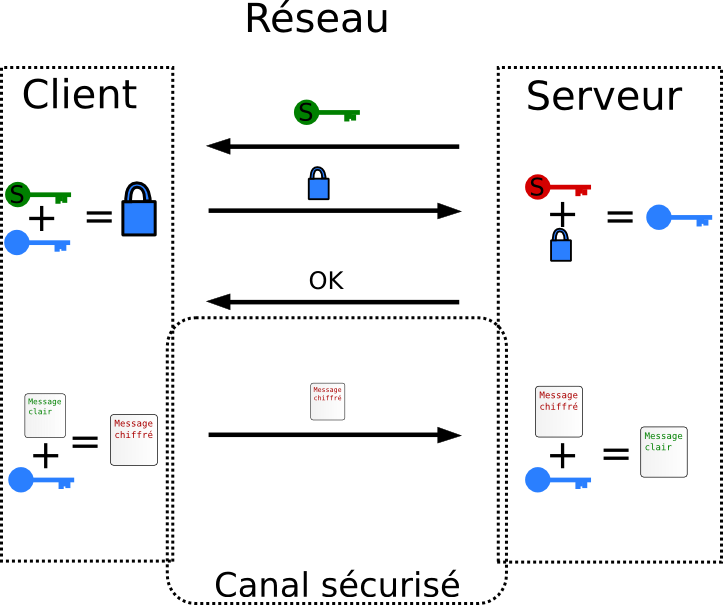
\includegraphics[width=0.4\textwidth]{images/SSH.png}}
    \hspace{1.2cm}
    \subfloat[Puffy, la mascotte du projet OpenBSD et de OpenSSH a
été 
choisie d'après l'algorithme \emph{blowfish} utilisé dans
OpenSSH, qui lui-même tire son nom du poisson-globe, représentant
la sécurité, la résistance aux attaques.]{
      \label{fig:Puffy}
\includegraphics[width=0.4\textwidth]{images/Puffy.png}}
    \caption{SSH}
    %\vspace{-15pt}
%  \label{fig:ScytaleChiffreCesar}
\end{figure}

Ensuite, l'authentification se fait la plupart du temps via un
simple nom d'utilisateur et mot de passe, mais peut se faire via
l'utilisation d'un chiffrement asymétrique : le serveur chiffre un message 
avec la clé
publique du client, et si celui ci parvient à le déchiffrer, il
sera identifié.
